% !TEX encoding = UTF-8 Unicode
\chapter{Les \mt clustering}
\label{chap3}
\section{Distance entres les \st}
Les s\'eries temporelles sont des données dans le temps et leur ordonnancement a une signification que l'on ne peut ignorer.  Ainsi, on ne peut pas leur appliquer des méthodes de fouille de données classiques qui supposent l’indépendance entre les exemples mais bien des méthodes spécialement adaptées, qui respectent la temporalité de ce type de donnée. 

Une mesure de distance entre deux séries temporelles peut être utilisée dans plusieurs tâches de data mining tel que l’apprentissage supervisé et l’apprentissage non supervisé. Dans les bases de données traditionnelles, les mesures de similarité sont basées sur un matching exact. Cependant, dans les données des séries temporelles, caractérisées par leur nature numérique et continue, la mesure de similarité est calculé d’une manière approximative.
Nous présentons ici quelques mesures de similarités entre deux séries temporelles :
\subsection{Distance Euclidienne}
La distance Euclidienne est une distance géométrique dans cet espace multidimensionnel qui ont beaucoup utilisé dans l’espace Euclidien. Un espace euclidien est un objet algébrique permettant de de généraliser de façon naturelle la géométrie traditionnelle développée par Euclide.
La distance Euclidienne est calculé comme étant : 
$$ d_{ED(u,v)} = \sqrt{ \frac{1}{N} \sum^{N}_{i = 1} {(u_i  - v_i)^2} }  $$
donc $u$ et $v$ sont des vecteurs de taille $N$. Comme la mesure de similarité ED n’a pas de borne supérieure et que sa valeur augmente avec le nombre de descripteurs N, il est conseillé de calculer la distance ED normalisée. De plus, cette distance ignore les dépendances temporelles entre les différentes séries de données. Ces deux contraintes ne permettent pas de comparer la forme du signal. 
\subsection{Complexe invariance distance -  CID}
La distance CID introduit par Keogh en 2011\cite{batista2011}, propose une notion plus robuste que la
distance euclidienne, car elle comporte un facteur de correcteur que nous pouvons associer à une
nouvelle mesure de dissimilarité. La distance CID est calculer par :
$$ d_{CID(u,v)} = 	d_{ED(u,v)}  \frac{max\{CE(u), CE(v) \} }  {min\{CE(u), CE(v) \} } $$
avec 
$$CE(x) = \sqrt{ \sum^{N-1}_{i = 1} {(x_i  - x_{i-1})^2} }    $$

$CE(x)$ est l’estimation de la complexité de la série temporelle x. Le facteur de complexité étant calculé en cumulant l’ensemble des variations locales du signal.
\subsection{Dynamic times wrapping - DTW}
Dans le domaine des données énergétiques, de nombreuses études portent sur la comparaison des mesures à différents endroits du bâtiment. A cause du phénomène de propagation de la chaleur, les signaux mesurant une même grandeur physique sont décalés dans le temps. Pour résoudre le problème de distorsion dans les séries temporelles, San- koffet Kurskal \cite{kruskal1983} ont présenté la distance de déformation temporelle “Dynamic Time Warping (DWT)” qui considère que le temps est élastique et non pas linéaire.

La distance DTW permet de comparer deux séries temporelles de dimension différente. Le principe de la distance consiste à mettre en correspondance les sous-séquences qui "se ressemblent" même si elles ne correspondent pas à un même intervalle de temp. La particularité de la méthode Dynamic Time Warping (DTW ) ou déformation dynamique temporelle, est de savoir gérer les décalages temporels qui peuvent éventuellement exister entre deux séries. Au lieu de comparer chaque point d’une série avec celui de l’autre série qui intervient au même instant t, on permet à la mesure de comparer chaque point d’une série avec un ou plusieurs points de l’autre série, ceux-ci pouvant être décalés dans le temps. 

La comparaison de deux séries temporelles U et V de dimensions respectives $m$ et $n$, est basée sur la réplication des valeurs jusqu’à l’obtention de la meilleure correspondance. Pour calculer la matrice de distance $(m x n)$, on initiale $d_{cum}(1,1) = | u_1 - v_1 |$. Après, on effectue l'initialisation de la premier ligne et la premier colonne de la matrice distance : 
$$d_{cum}(1, j) = | u_j - v_1 | + d_{cum}(1, j - 1) , pour j > 1$$ 
$$d_{cum}(i, 1) = | u_1 - v_i | + d_{cum}(i - 1, j),  pour  i > 1$$ 
Les valeurs des autres cases sont calculées comme suites pour $i + j > 2$ : 
$$d_{cum}(i, j) = d_{ED(u, v)} + min \{  d_{cum}(i - 1, j), d_{cum}(i, j - 1), d_{cum}(i - 1, j - 1) \} $$
Pour relier les point U et V, il faut trouver le chemin qui minimise la distance cumulé. Cet chemin W est formé de K point avec $max(m,n) \leq K \leq n + m – 1$. La distance DWT optimale est :
$$d_{DWT(U, V)} = min\sqrt{\sum^{K}_{k = 1} {d_{ED(k)}}} $$
Selon ce principe, la DTW a tendance à expliquer les variations de l’axe des Y en déformant l’axe des X. Cela peut cependant induire à des alignements non désirables.
\subsection{Derivative dynamic times wrapping - DDTW}
La distance DTW a tendance à expliquer les variations de l’axe des Y en déformant l’axe des X. Cela peut cependant induire à des alignements non désirable. Pour répondre à cette problème, Keogh et Pazzani ont proposé en 2001 une modification de la DTW nommée “Derivative Dynamic Times Warping (DDTW) \cite{keogh2001}. 

Cette méthode prend en compte la forme des séries temporelles et de la premier dérivée des séquences. Le premier terme dans le calcul de la distance cumulée n’est plus celui de la distance Euclidienne $d_{ED} (u_i  - v_i)$, mais celui de l’estimation de la dérivée de $u_i$ et $v_i$ :
$$d_x(v_i) = \frac{(v_i - v_{i - 1}) + \frac{(v_{i + 1} - v{i - 1} )} {2}    } {2} $$
La distance DDTW fournit des performances nettement supérieurs à celle de la DWT original en minimisant le nombre les point dupliqués.
\subsection{Adaptive Feature Base Dynamic Time Warping }
Les distances DTW et DDTW ne permettent pas de trouver un alignement dans le cas de données manquantes, ce qui est très fréquent dans les mesures réelles. Xie et Wiltgen a présenté la méthode “Adaptive Feature Base Dynamic Time Warping (AFBDTW)” en 2010 \cite{xie2010} permet de prendre en compte à la fois le caractère local ainsi que global des séries pour les correspondances au lieu de la valeur elle même ou de sa dérivée.

Le caractère locale de $u_i$ nommé $f_{local}(i)$ est définit par : 
$$f_{local}(i) = (u_i - u_{i-1}, u_i - u_{i+1} )$$

Il semblerait que cette définition représente d’une meilleure façon le caractère global par rapport à la dérivée de la DDTW. Le caractère global est défini par :
$$f_{global}(i) = (u_i - \frac{1}{i-1} \sum_{k = 1}^{i - 1} {u_k}, u_i -  \frac{1}{m - i} \sum_{k = i + 1}^{m} {u_k} ) $$

Pour évaluer la distance entre $u_i$ et $v_j$, on définit $dist(u_i, v_j)$ comme suit. Le calcul de $d_{cum}$ restera le même que celui définit précédemment.
$$dist(u_i, v_j) = W_1 \bullet dist_{local} (u_i, v_j) + W_2 \bullet dist_{global}(u_i, v_j)$$
avec 
$$dist_{local} (u_i, v_j) = | (f_{local}(u_i))_1 - (f_{local}(v_j))_1  | + | (f_{local}(u_i))_2 - (f_{local}(v_j))_2  | $$
$$dist_{global}(u_i, v_j) = | (f_{global}(u_i))_1 - (f_{global}(v_j))_1  | + | (f_{global}(u_i))_2 - (f_{global}(v_j))_2  | $$
$$W_1 + W_2 = 1 \hspace{1cm} 0 \leq W_1 \leq 1 \hspace{1cm} 0 \leq W_2 \leq 1$$

Les poids $W_1$ et $W_2$ permettent de régler le pourcentage d’influence du critère local et global. La classification des séries temporelles basée sur la mesure de similarité avec la AFBDTW, est le meilleur compromis, permettant de prendre en compte à la fois le critère local et global des séries temporelles.
\subsection{Fast time series evaluation - FTSE}
La méthode FTSE a été présenté par M. Morse et Jignesh M. Patel \cite{morse2007} est une technique pour évaluer la seconde classe de fonctions de comparaison de la série de temps qui calculent un score de similarité basé sur un seuil correspondant.

Cette méthode identifies les éléments d’adaptation $u_i$ et $v_j$ entre deux séries temporelles $U$ et $V$ sans utilisant les grandes matrices à deux dimension. Ceci est réalisé en traitant $U$ et $V$ de manière non uniforme, plutôt que de les traiter de la même façon que dans la programmation dynamique.

Pour trouver les paires entre $U$ et $V$ sans comparer chaque $u_i$ avec chaque $v_j$, la méthode FTSE indices les éléments de $U$ sur une grille. Chaque élément de $U$ est placée dans une cellule de la grille. Maintenant, pour trouver les éléments de $U$ qui correspond $v_j$, la grille est sondée avec $v_j$. Seuls les éléments de $U$ qui résident dans la même cellule de
grille comme $v_j$ doivent être comparés avec elle pour voir si elles correspondent.

FTSE mesure la similarité entre les séries temporelles $U$ et $V$ avec une valeur de seuil $\varepsilon$. En utilisant $\varepsilon$, chaque paire d'élément $u_i \in U$ et $v_j \in V$ peut être classer comme un match ou on décalage. On peut dit un élément $u_i$ et $v_j$ est match si $| u_i - v_j | <  \varepsilon$ dans tous dimensions.

On a montré que la traitement de FTSE a beaucoup plus vite que la traitement des méthode traditionnelle qui utilise la programmation dynamique (comme DTW).
\subsection{K-means clustering}
K-means clustering est une méthode de quantification vectorielle, à l'origine du traitement du signal, qui est populaire pour l'analyse de cluster dans l'exploration de données. K-means clustering vise à partitionner $n$ observations en $k$ clusters dans lesquels chaque observation appartient au cluster avec la moyenne la plus proche, sert de prototype du cluster. L'idée principale est la minimisation d'une fonction objective, qui est normalement choisie comme étant la distance totale entre tous les modèles de leurs centres de cluster respectifs. Sa solution repose sur un schéma itératif, qui commence par des appartenances ou des centres de cluster initiaux choisis arbitrairement. La répartition des objets entre les clusters et la mise à jour des centres de clusters sont les deux principales étapes de l'algorithme c-means. L'algorithme alterne entre ces deux étapes jusqu'à ce que la valeur de la fonction objectif ne puisse plus être réduite.

Étant donné n motifs $ \{ x_k | k = 1,...., n\}$, k-means détermine $c$ centres de cluster $\{ v_i | i = 1,..., c\}$, en minimisant la fonction objectif donnée comme : 
$$Min J_1(U, V) = \sum_{i = 1}^{c} \sum_{k = 1}^{n} u_{ik} \parallel x_k - v_i \parallel ^2 $$
avec 
$$u_{ik} \in \{0, 1\} \forall i,k \hspace{1cm} \sum_{i = 1, c} u_{ik} = 1, \forall k$$
et $\parallel \bullet \parallel$ dans l'équation ci-dessus est normalement la mesure de distance euclidienne entre les séries temporelles. Cependant, d'autre mesure de distance pourraient également être utilisées. La procédure de solution itérative comporte généralement les étapes suivants : 
\begin{itemize}
\item[(1)] Choisit c ($2 \leq c \leq n$) et $\varepsilon$ (un petit nombre pour arrêter la procédure itérative). Régler le compteur $l = 0$ et initialiser les centres des cluster $V^(0)$ arbitrairement.
\item[(2)] Distribué $x_k, \forall k $ pour déterminer $U^{(l)}$ de sorte que $J_1$ soit minimisé. Ceci est réalisé normalement en réaffectant $x_k$ à un nouveau cluster qui en est le plus proche.
\item[(3)] Révisé les centres des cluster $V^(l)$
\item[(4)] Arrêté si le changement de $V$ est plus petit que $\varepsilon$. Sinon, augmenté $l$ et répété les étapes 2 et 3.
\end{itemize}

Bien qu'il puisse être prouvé que la procédure se terminera toujours, l'algorithme k-means ne trouve pas nécessairement la configuration la plus optimale, correspondant à la fonction objective globale minimum. L'algorithme est également sensible aux centres de clusters sélectionnés au hasard. L'algorithme k-means peut être exécuté plusieurs fois pour réduire cet effet.

K-means est un algorithme simple qui a été adapté à de nombreux domaines problématiques. Comme nous allons le voir, c'est un bon candidat pour que l'extension fonctionne avec des vecteurs de fonctions flous.
\section{ Analysis de Silhouette}
L'analyse de Silhouette est une méthode d'interprétation et de validation de la cohérence au sein de groupes de données \cite{rousseeuw1987}. Cette technique fournit une représentation graphique succincte de la façon dont chaque objet se trouve dans son groupe. La valeur de silhouette est une mesure de la similitude entre un objet et son propre cluster (cohésion) par rapport aux autres clusters (séparation). La silhouette valeur varie de -1 à +1, où une valeur élevée indique que l'objet est bien adapté à son propre cluster et mal adapté aux clusters voisins. Si la plupart des objets ont une valeur élevée, la configuration de cluster est appropriée. Si de nombreux points ont une valeur faible ou négative, la configuration de clustering peut comporter trop ou trop peu de clusters.

Supposer que les données ont été regroupées par n'importe quelle technique, tel que k-means, en $k$ clusters. Pour chaque donnée $i$, soit $x(i)$ la distance moyenne entre $i$ et toutes les autres données dans le même groupes. Nous définissons ensuite la dissimilarité moyenne du point $i$ à un cluster $c$ comme la moyenne de la distance de $i$ à tous les points de $c$.

Soit $y(i)$ la distance moyenne la plus basse de $i$ à tous les points de tout autre groupe, dont $i$ n'est pas membre. Le cluster avec cette dissimilarité moyenne la plus basse est dit le "cluster voisin" de $i$ parce que c'est le cluster suivant le plus approprié pour le point $i$. Nous définissons maintenant une silhouette: 
$$s(i) = \frac{y(i) - x(i)}{max\{ x(i), y(i)\}}$$
On peut aussi écrit comme : 
$$s(i) = \left\{ 
\begin {tabular}{c c}
1 - x(i)/y(i) & si x(i) < y(i) \\
0, & si x(i) = y(i)\\
y(i)/x(i) - 1 & si x(i) > y(i)
\end{tabular}
\right.$$
Il est très claire que $-1 < s(i) < 1$. Si $s(i)$ soit plus proche 1, alors $x(i)\ll y(i)$. Comme $x(i)$ est la mesure de la distance moyenne de $i$  à son cluster, une petite valeur signifie qu'il est bien groupé. De plus, un grand $y(i)$ implique que $i$ est mal groupé à son cluster voisin. Ainsi, un $s(i)$ proche de 1 signifie que les données sont regroupées de manière appropriée.Si $s(i)$ est proche de négatif, alors par la même logique nous voyons que je serais plus approprié s'il était groupé dans son cluster voisin. Un $s(i)$ proche de zéro signifie que la donnée est à la frontière de deux groupes naturels. 
\section{Clustering les données de la dengue}
Dans cette partie, nous avons appliqué la méthode k-means pour grouper les données de la dengue des provinces des pays dans la région Asie du Sud-Est. Nous utilisons les taux d'inflection des pays Vietnam, Laos, Cambodge, Malaisie, Philippines, Thaïlande, Singapour et Taiwan à partir de Janvier 1998 jusqu'au Septembre 2010 pour effectuer le k-means. Les données des provinces de l'Indonésie n'était  pas  être utilisés à cause de la carence et de la discontinuité. La distance entre les séries temporelles des provinces sont calculés par la méthode DTW. La méthode d'analyse silhouette a été utilisé pour évaluer le nombre des cluster de la méthode k-means. Le tableau 3.1 montre les silhouettes coefficients (SE) des différents nombres de cluster (NC) de la méthode k-means. On trouve que le nombre de cluster qui a eu la valeur silhouette le plus mieux est égal à 3. Nous avons appliqué la méthode k-means pour grouper les taux d'infections des provinces des pays et leurs visualisation sont présenté sur la figure \ref{Pic3_1}.  On a traité un test spatial pour évaluer le résultat de la méthode k-means. On a calculé la distance moyenne entre les provinces dans le même groupe en utilisant leurs latitude et longitude. Puis on va créer des séquences de résultats générée aléatoirement en classant les provinces dans les groupes aléatoire. Ensuite on calcule les distances moyennes de ces séquences et leur compare avec celui de la méthode k-means pour obtenir valeur statistique. La figure \ref{Pic3_2} montre la résultat du test statistique de la méthode k-means avec k = 3 et le nombre de répétition des séquence aléatoires est 1.000.000 fois. On a trouvé le p-valeur : $p < 1e-6$ et ceci est une résultat très significatif.

Ce résultat suggère que la catégorisation des provinces  basée sur la situation de la dengue entre janvier 1998 et septembre 2010 par l'algorithme k-means a donné un très bon résultat lorsque la distance moyenne entre les provinces d'un même groupe est révélée optimale. On peut facilement détecter les région commune comme : Le Nord du Vietnam et de Laos, le centre du Vietnam et de Laos, l'Ouest de Laos et de Thaïlande, le Sud du Vietnam et du Cambodge, le Taiwan, le Philippines, L'est du Malaisie. En raison de la proximité de géographique, ces zones peuvent avoir les mêmes conditions générales de climat. Si les facteurs météorologiques influencent le développement de la dengue, la  distribution des provinces sur les cluster dans la figure \ref{Pic3_1} est également relativement appropriée. Cela signifie que la situation épidémique des villes voisines peut être influencée par les autres ou affectée par les mêmes conditions météorologiques et géographiques. Dans les chapitre après nous allons identifier la relation entre les facteurs environnementaux et l'infection de la dengue par les différentes méthodes.
\begin{table}[h]
\centering
\begin{tabular} { | c | c |}
\hline
Nombre de cluster & Silhouette coefficient \\
\hline
2 & 0.5734565 \\
\hline
3 & 0.581752 \\
\hline
4 & 0.5420058 \\
\hline
5 & 0.5307371 \\
\hline
6 & 0.5148082 \\
\hline
7 & 0.4907725 \\
\hline
8 & 0.4794107 \\
\hline
9 & 0.4964826 \\
\hline
10 & 0.4867265 \\
\hline
11 & 0.4732487 \\
\hline
12 & 0.472837 \\
\hline
13 & 0.484026 \\
\hline
14 & 0.473134 \\
\hline
15 & 0.4924166 \\
\hline
16 & 0.4496414 \\
\hline
17 & 0.4425588 \\
\hline
18 & 0.4652832 \\
\hline
19 & 0.4520348 \\
\hline
20 & 0.4081333 \\

\hline
\end{tabular}
\caption{Silhouette coefficient des différents valeurs de clusters} 
\label{table3.1}
\end{table}

\begin{figure}[h]
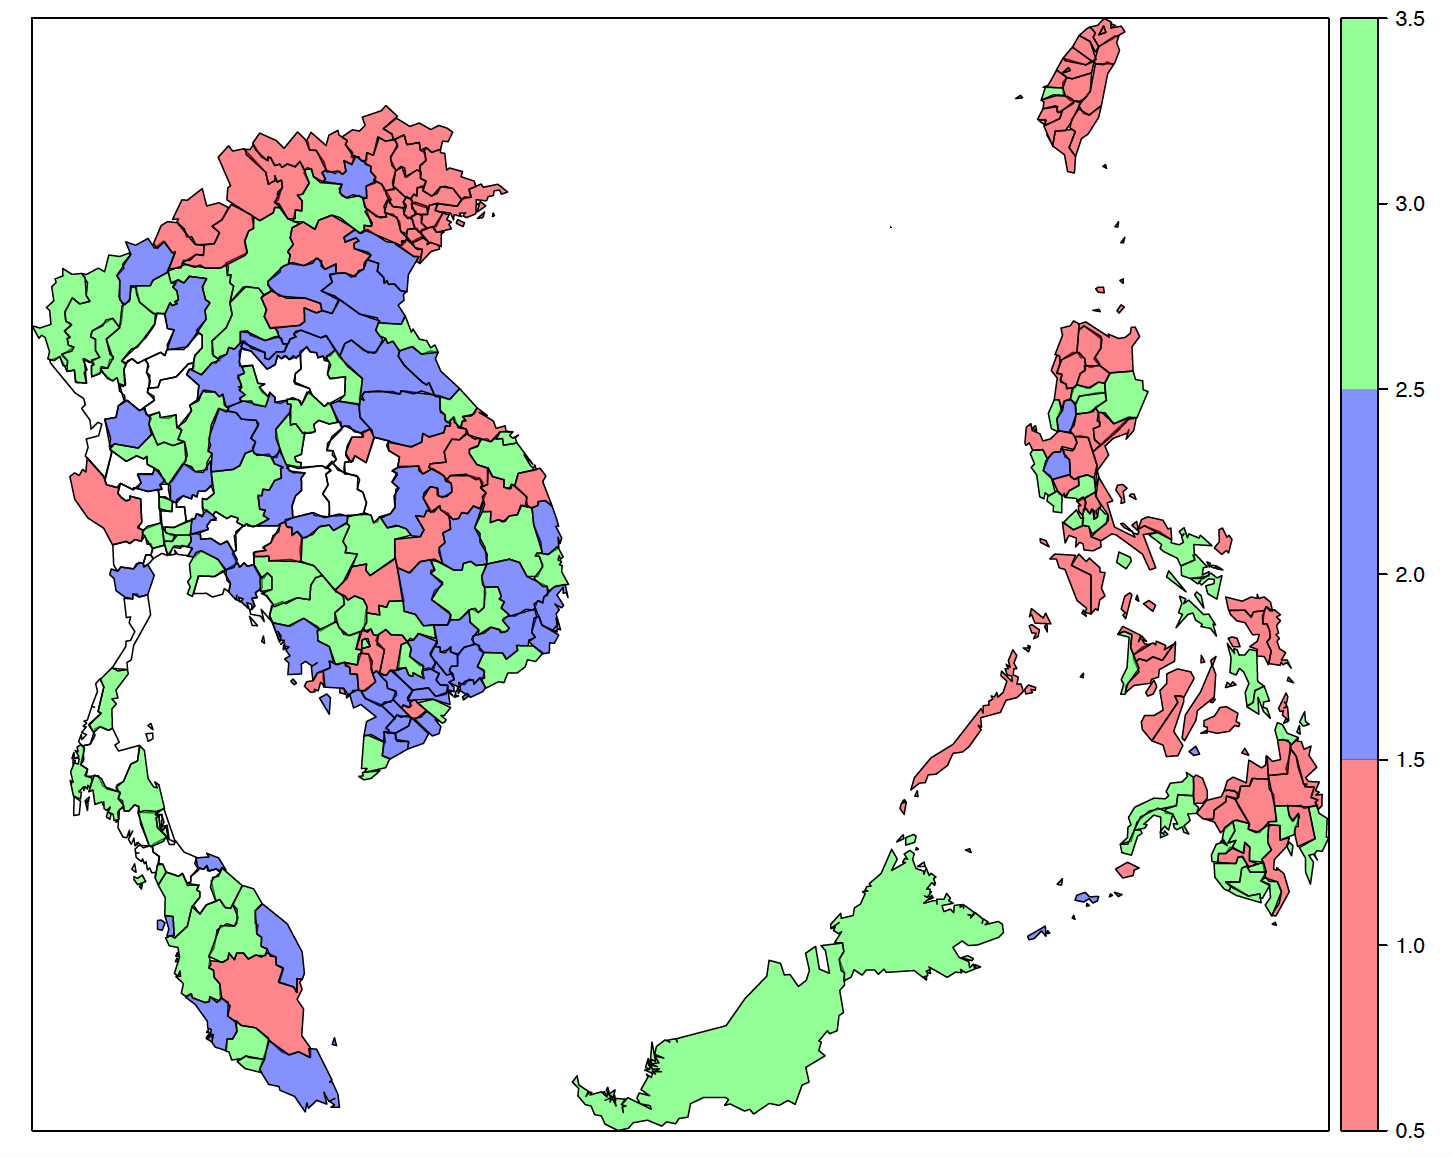
\includegraphics[width = \linewidth]{../figures/chap3/Pic3_1.png}
\caption{Résultat de la méthode k-means avec k = 3, méthode validation : silhouette}
\label{Pic3_1}	
\end{figure}

\begin{figure}[h]
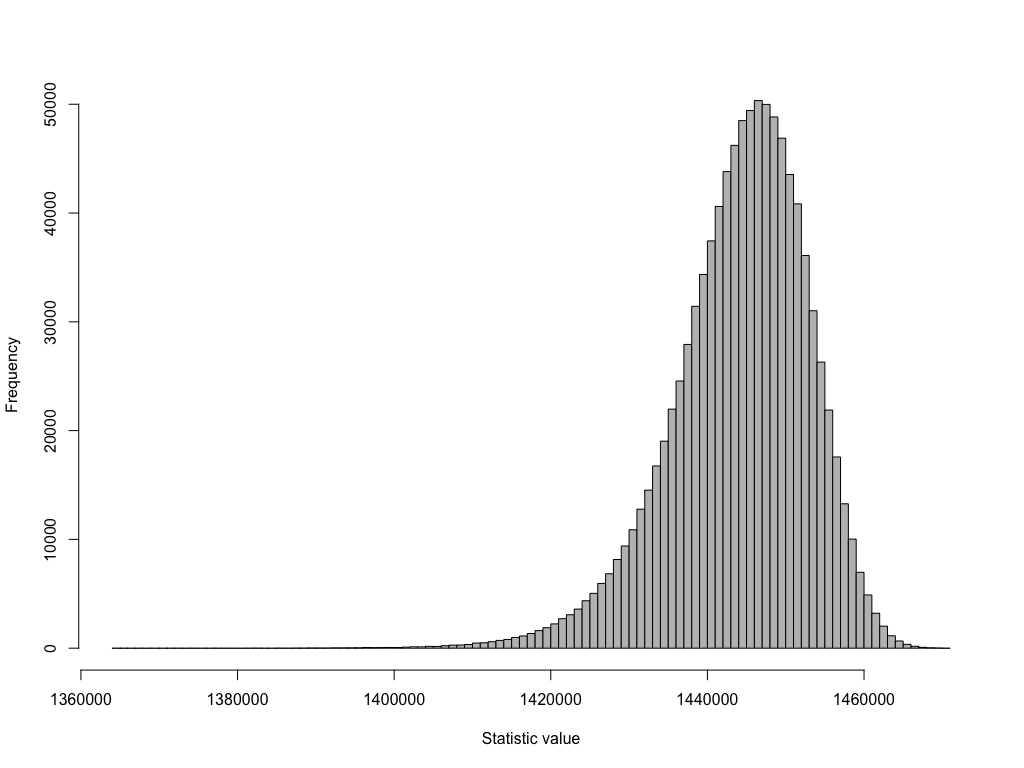
\includegraphics[width = \linewidth]{../figures/chap3/Pic3_2.png}
\caption{Résultat du test statistique de la méthode k-means avec k = 3}
\label{Pic3_2}	
\end{figure}
